\documentclass{article}

\usepackage{graphicx}
\usepackage{tikz}
\usepackage{tikzsymbols}
\usetikzlibrary{calc,patterns,shapes.geometric}
\pagestyle{empty}
\usepackage[margin=0pt]{geometry}
\geometry{papersize={14in,12in}}

\def\centerarc[#1](#2)(#3:#4:#5){\draw[#1] ($(#2)+({#5*cos(#3)},{#5*sin(#3)})$) arc (#3:#4:#5);}

\begin{document}
	\begin{figure}
		\centering
		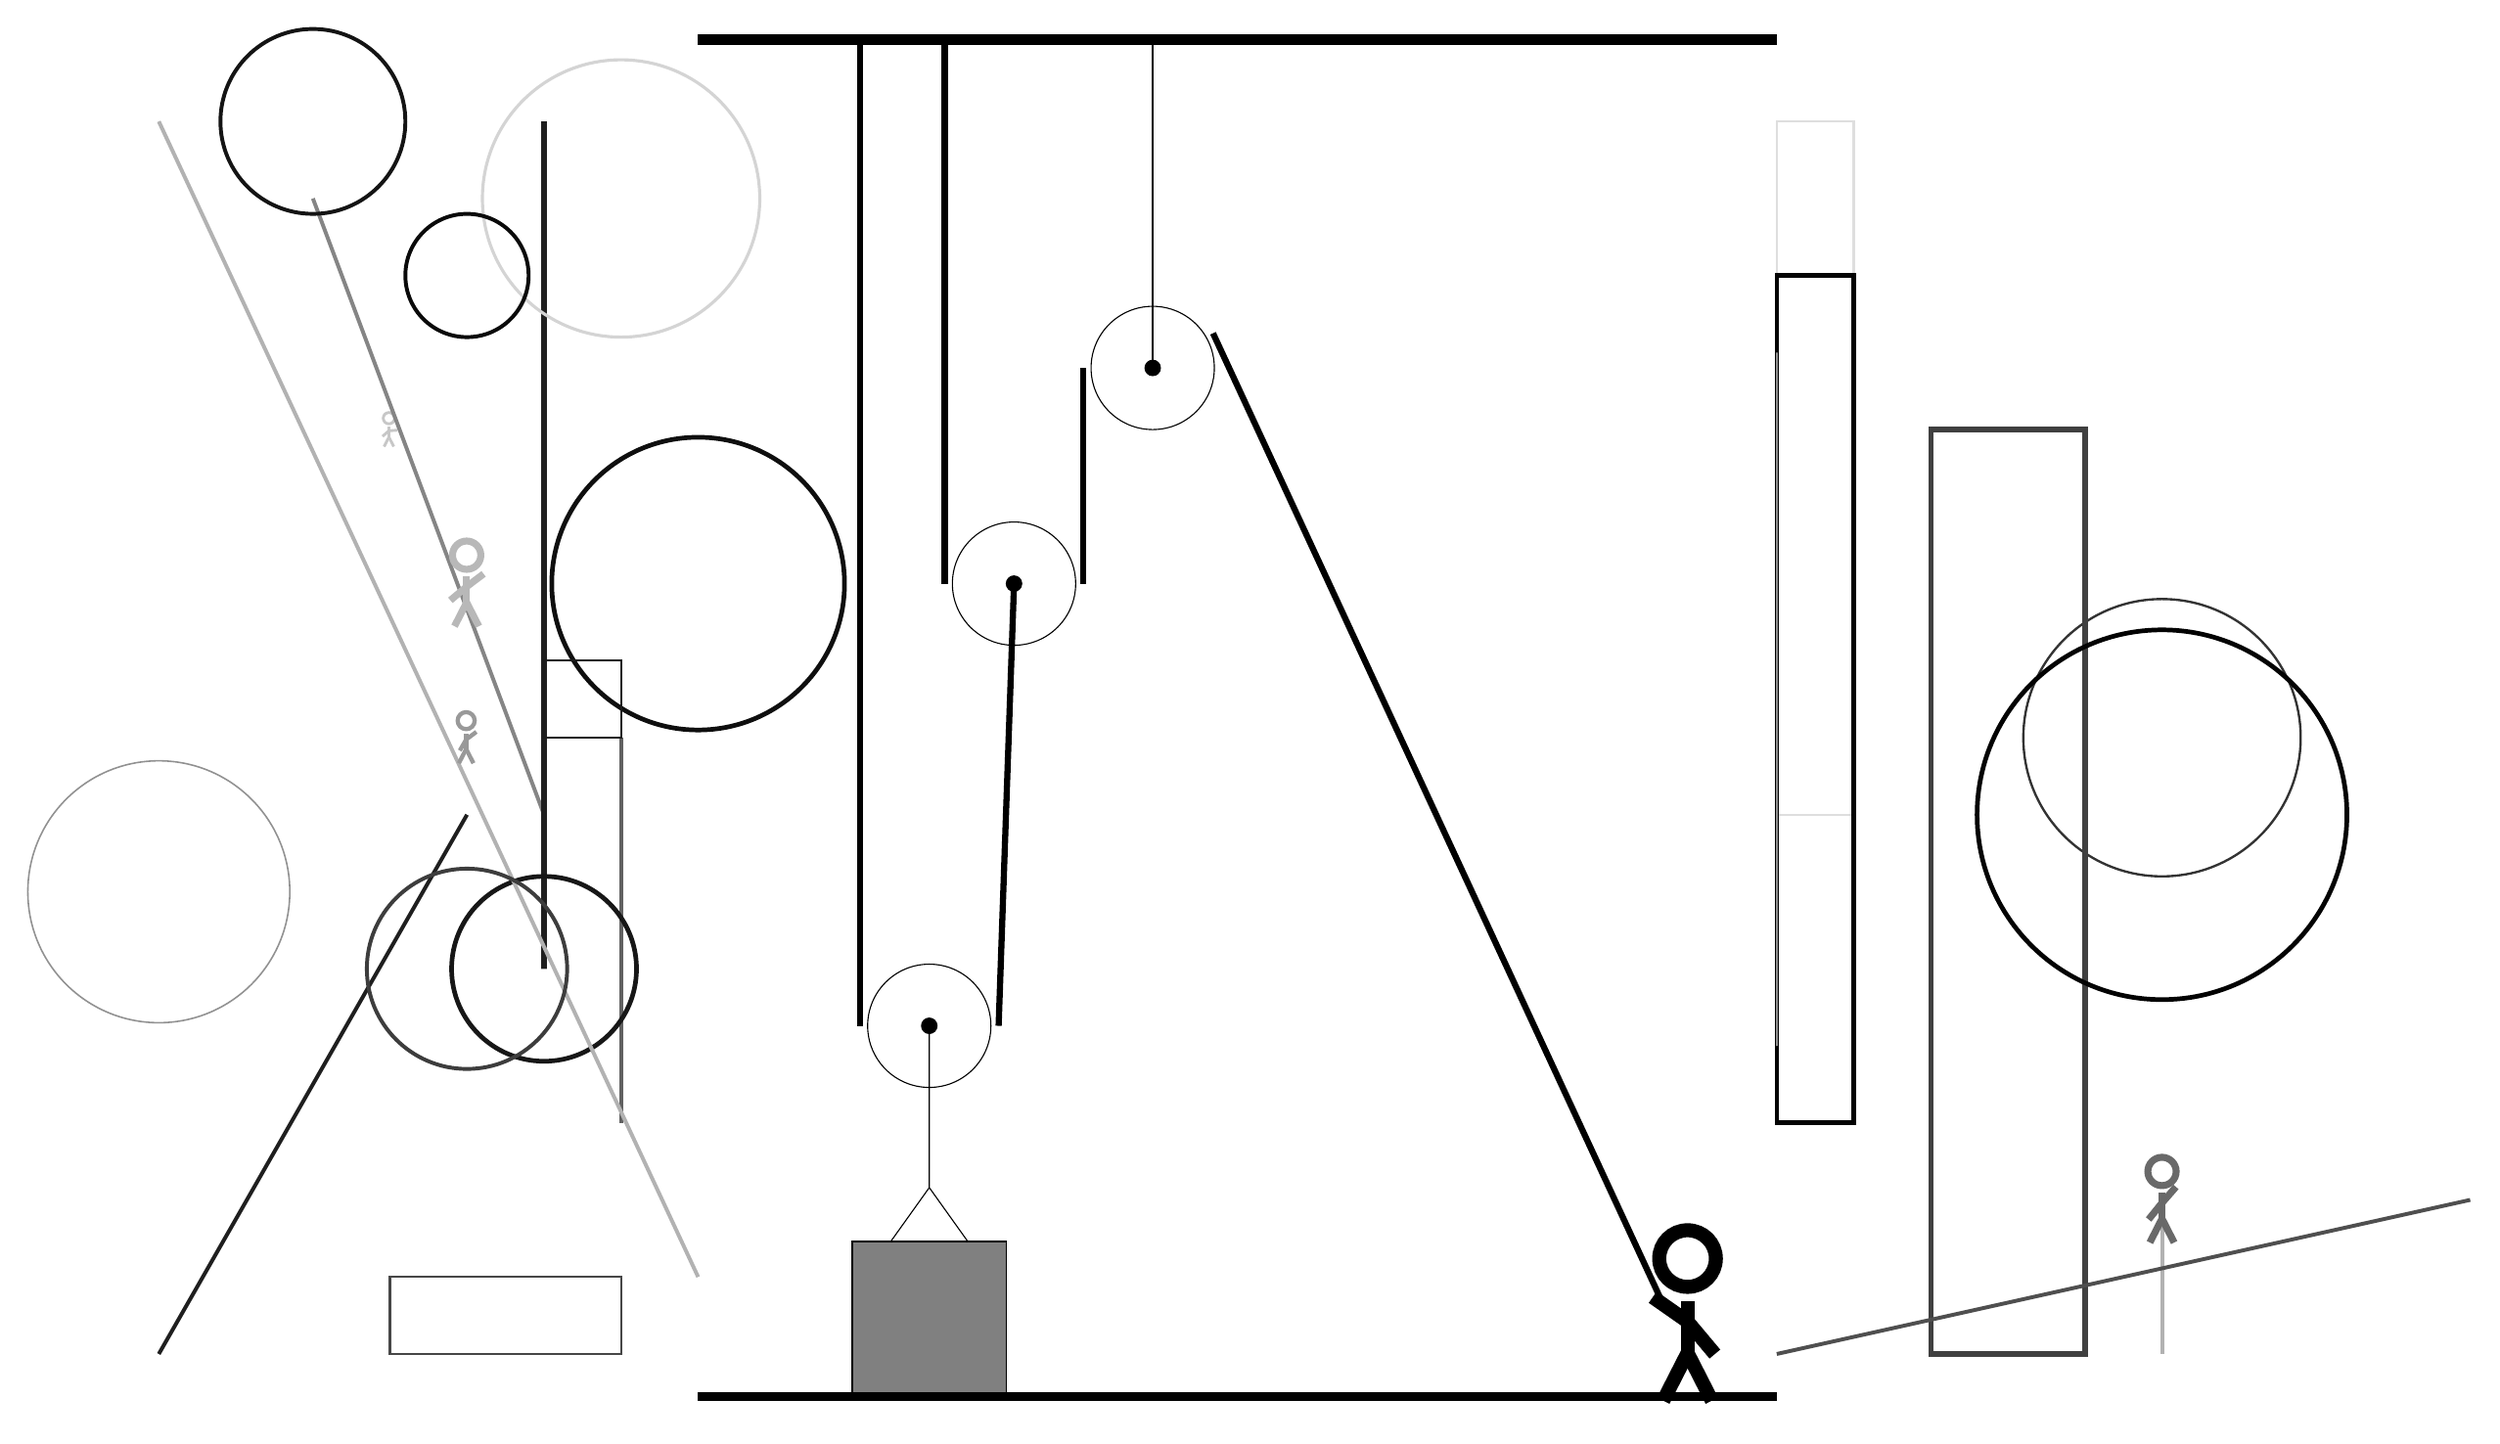
\begin{tikzpicture}
			%%%%% START %%%%%
			
			\draw[fill=black] (-2, 14) rectangle (12, 14.125);
			
			\draw (1, 1.26) circle (0.8);
			\draw[fill=black] (1, 1.26) circle (0.1);
			
			\draw (2.1, 7.0) circle (0.8);
			\draw[fill=black] (2.1, 7.0) circle (0.1);
			
			\node[line width=0.6mm, color=black!22] at (-6, 9) {\Strichmaxerl[2][41][4]};
			
			\draw [line width=0.2mm, color=black!43](-9, 3) circle (1.7);
			\draw[line width=0.5mm, color=black!48](-4, 4) -- (-7, 12);
			\draw[line width=0.7mm, color=black!88] (-4, 13) rectangle (-4, 2);
			
			\draw[line width=0.3mm, color=black!13] (13, 4) rectangle (12, 13);
			\draw [line width=0.7mm, color=black!87](20, 13) circle (0.0);
			\draw [line width=0.3mm, color=black!80](17, 5) circle (1.8);
			
			\draw[line width=0.5mm, color=black!62] (-3, 5) rectangle (-3, 0);
			\draw [line width=0.4mm, color=black!17](-3, 12) circle (1.8);
			
			\draw[line width=0.5mm, color=black!88](-5, 4) -- (-9, -3);
			
			\draw[line width=0.7mm, color=black!75] (14, 9) rectangle (16, -3);
			
			\draw[line width=0.6mm, color=black!99] (12, 11) rectangle (13, 0);
			\draw [line width=0.5mm, color=black!96](-5, 11) circle (0.8);
			
			\draw [line width=0.6mm, color=black!91](-4, 2) circle (1.2);
			\draw[line width=0.5mm, color=black!30](-2, -2) -- (-9, 13);
			\draw[line width=0.5mm, color=black!30](17, -3) -- (17, -1);
			
			\draw[line width=0.3mm, color=black!72] (-3, -2) rectangle (-6, -3);
			\node[line width=0.4mm, color=black!40] at (-5, 5) {\Strichmaxerl[3][60][37]};
			\draw [line width=0.6mm, color=black!94](-2, 7) circle (1.9);
			\node[line width=0.2mm, color=black!28] at (-5, 7) {\Strichmaxerl[5][40][37]};
			\draw [line width=0.5mm, color=black!76](-5, 2) circle (1.3);
			
			\draw[line width=0.5mm, color=black!69](12, -3) -- (21, -1);
			\node[line width=0.4mm, color=black!59] at (17, -1) {\Strichmaxerl[5][51][49]};
			\draw[line width=0.2mm, color=black!44] (12, 1) rectangle (12, 10);
			\draw [line width=0.5mm, color=black!92](-7, 13) circle (1.2);
			\draw [line width=0.6mm, color=black!99](17, 4) circle (2.4);
			
			\draw[line width=0.3mm, color=black!89] (-3, 6) rectangle (-4, 5);
			
			\draw (3.9, 9.8) circle (0.8);
			\draw[fill=black] (3.9, 9.8) circle (0.1);
			\draw[thick] (3.9, 9.8) -- (3.9, 14);
			
			\draw (1, 1.26) -- (1, -0.84) -- (0.5, -1.54) -- (1.5, -1.54) -- (1, -0.84);
			\draw[fill=black!50] (0, -1.54) rectangle (2, -3.54);
			
			\draw[line width=0.8mm] (0.1, 14) -- (0.1, 1.26);
			\centerarc[line width=0.8mm](1, 1.26)(180:360:0.9);
			\draw[line width=0.8mm](1.9, 1.26) -- (2.1, 7.0);
			\draw[line width=0.8mm] (1.2, 14) -- (1.2, 7.0);
			\centerarc[line width=0.8mm](2.1, 7.0)(180:360:0.9);
			\draw[line width=0.8mm](3.0, 7.0) -- (3.0, 9.8);
			\centerarc[line width=0.8mm](3.9, 9.8)(30:180:0.9);
			\draw[line width=0.8mm] (4.683, 10.25) -- (10.5, -2.3);
			
			\node at (10.8, -2.5) {\Strichmaxerl[10][-35][-50]};
			
			\draw[fill=black] (-2, -3.5) rectangle (12, -3.6);
			
			%%%%% END %%%%%
		\end{tikzpicture}
	\end{figure}	
\end{document}